
\section{Introduction}\label{sec:intro}
The sequence of Catalan numbers $\{C_n\}_{n\geq0}$ is one of the most well-studied sequences in combinatorics. They have a product formula $C_n=\binom{2n}{n}/(n+1)$ and count Dyck paths, binary trees, triangulations and many more classical combinatorial objects \cite{stanley2015catalan}. In this paper, we focus on weighted Catalan numbers, one of the many generalizations of Catalan numbers, and their arithmetic.

Recall that a \textit{Dyck path} of semilength $n$ is a sequence of points $\{(x_k,y_k)\}_{k=0}^{2n}$ that starts at $(x_0,y_0)=(0,0)$ and ends at $(x_{2n},y_{2n})=(2n,0)$  in the upper half-plane of the integer lattice $\Z^2$ such that each step $s_k=(x_{k}-x_{k-1},y_{k}-y_{k-1})$ is either $(1,-1)$ or $(1,1)$. For a fixed sequence of integers $b=(b(0),b(1),b(2),\ldots)$, define the \textit{weight} of a step $s_k$ to be $b(y_{k-1})$ if $s_k$ has the form $(1,1)$ and 1 if $s_k$ has the form $(1,-1)$. For a Dyck path $P$, define its \textit{weight} $\wt_b(P)$ to be the product of the weights of its steps. See Figure~\ref{fig:dyckpath} for an example.
\begin{figure}[h!]
\centering
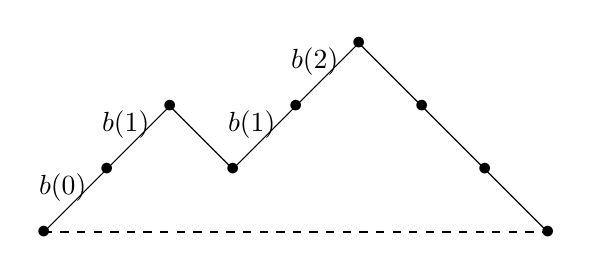
\begin{tikzpicture}[scale=0.8]
\node at (0,0) {$\bullet$};
\node at (1,1) {$\bullet$};
\node at (2,2) {$\bullet$};
\node at (3,1) {$\bullet$};
\node at (4,2) {$\bullet$};
\node at (5,3) {$\bullet$};
\node at (6,2) {$\bullet$};
\node at (7,1) {$\bullet$};
\node at (8,0) {$\bullet$};
\node at (0.3,0.7) {$b(0)$};
\node at (1.3,1.7) {$b(1)$};
\node at (3.3,1.7) {$b(1)$};
\node at (4.3,2.7) {$b(2)$};
\draw(0,0)--(2,2)--(3,1)--(5,3)--(8,0);
\draw[dashed](0,0)--(8,0);
\end{tikzpicture}
\caption{A Dyck path with weight $b(0)b(1)^2b(2)$.}
\label{fig:dyckpath}
\end{figure}
\begin{definition}
For $b:\Z_{\geq0}\rightarrow\Z$, the \textit{weighted Catalan numbers} $C_n^b$ are defined as
\[C_n^b=\sum_{P}\wt_b(P)\]
where the sum is over all Dyck paths $P$ of semilength $n$ and the weight of a Dyck path, $\wt_b(P)$, is explained as above.
\end{definition}
The weighted Catalan numbers have a beautiful generating function, illustrated in the following proposition, which is left as a simple exercise for the reader, whose proof can be found in the book of Goulden and Jackson \cite{goulden2004combinatorial}.
\begin{proposition}
\label{prop:genfunc}
The weighted Catalan numbers have the following generating function:
\[\sum_{n\geq0}C_n^bx^n=\cfrac{1}{1-\cfrac{b(0)x}{1-\cfrac{b(1)x}{1-\cfrac{b(2)x}{1-\cdots}}}}.\]
\end{proposition}
Specializations of weighted Catalan numbers count many interesting combinatorial objects. We provide some examples here. When $b\equiv1$, we recover the usual Catalan numbers. When $b(k)=k+1$, $C_n^b=(2n-1)!!$ counts the number of matchings of $2n$ objects. When $b(k)=(k+1)^2$, $C_n^b$ counts the number of alternating permutations of size $2n$ and when $b(k)=(k+1)(k+2)$, $C_n^b$ counts the number of alternating permutations of size $2n+1$ \cite{goulden2004combinatorial}. Finally, when $b(k)=(2k+1)^2$, $C_n^b$ counts the number of combinatorial types Morse links of order $n$ \cite{postnikov2000morse}.

The divisibility of Catalan numbers by powers of 2 has been determined both arithmetically and combinatorially (see for example \cite{dickson1966history} and \cite{deutsch2006congruences}). For a positive integer $q\geq2$ and for $n\in\Z_{>0}$, let $\xi_q(n)$ be the unique $m\in\Z_{\geq0}$ such that $q^m\mid n$ and $q^{m+1}\nmid n$ and let $s_q(n)$ be the sum of digits in the $q$-ary expansion of $n$. It is then well-known that $\xi_2(C_n)=s_2(n+1)-1$.

Postnikov and Sagan \cite{postnikov2007power} provided a sufficient condition on $b:\Z_{\geq0}\rightarrow\Z$ for $\xi_2(C_n^b)=\xi_2(C_n)$. For any function $f:\Z_{\geq0}\rightarrow\Z$, let $\Delta f:\Z_{\geq0}\rightarrow\Z$ be defined as $(\Delta f)(x)=f(x+1)-f(x)$.
\begin{theorem}[\cite{postnikov2007power}]\label{thm:postsagan}
If $b:\Z_{\geq0}\rightarrow\Z$ satisfies
\begin{enumerate}
    \item $b(0)$ is odd,
    \item $2^{n+1}\mid(\Delta^nb)(x)$ for all $x\in\Z_{\geq0}$,
\end{enumerate}
then $\xi_2(C_n^b)=\xi_2(C_n)=s_2(n+1)-1$ for all $n$.
\end{theorem}
In the case where $b$ is a polynomial function, a necessary and sufficient condition for $\xi_2(C_n^b)=\xi_2(C_n)$ for all $n$ was conjectured by Konvalinka \cite{konvalinka2007divisibility} and resolved by An \cite{an2010combinatorial} arithmetically. A generalization of Theorem~\ref{thm:postsagan} to weighted $q$-Catalan numbers, for a prime power $q$, is given by Konvalinka \cite{konvalinka2007divisibility}.

In this paper, we relax conditions of Theorem~\ref{thm:postsagan} and also arrive at the conclusion that $\xi_2(C_n^b)=\xi_2(C_n)$. Our main theorem is stated and proved in Section~\ref{sec:thm} using combinatorial arguments on binary trees. In Section~\ref{sec:generalization}, we show that a similar approach can be used to generalize our results to weighted $q$-Catalan numbers. In addition, in a different setting, we discuss modulo arithmetic of weighted Catalan numbers in Section~\ref{sec:period}, resolving some periodicity conjectures by Postnikov \cite{postnikov2000morse}. Many intriguing conjectures will be mentioned along the way.

